\documentclass[11pt,a4paper,oneside]{article}
\usepackage{calculator}
\usepackage{calculus}
\usepackage{amsthm}
\usepackage{amsmath}
\usepackage{cmtt}
\usepackage[dvips]{geometry}
\usepackage{pstricks}
\usepackage{graphicx}
\usepackage{graphics}
\usepackage{pst-plot}
\usepackage{pst-node}
\usepackage{multido}
\usepackage{pst-xkey}
\usepackage{pst-func}
\usepackage{pstricks-add}
\usepackage[pdftex,colorlinks,linktocpage]{hyperref}
\def\hantt{\^e}\def\accentcircflx{\hskip-.3em\raisebox{0.32ex}{\'{}}}
%%%%%%%%%%%%%%%%%%%%%%%%%%%%%%%%%%%%%%%%%%%%%%%%%%%%%%%%%%%%%%%%%%%%%%%%%%%%%%%%%%%%%%%%
\def\RiemannSum#1#2#3#4#5#6#7#8#9{%
\psplot[linecolor=blue]{#1}{#2}{#3}
\pscustom[linecolor=red]{%
\psline{-}(#1,0)(#1,0)
\multido{\ni=#5,\ne=#6}{#4}
{\psline(*{\ni} {#8})(*{\ne} {#9})}}
\multido{\ne=#6,\nc=#7}{#4}
{\psdot(*{\nc} {#3})
\psline[linestyle=dotted,dotsep=1.5pt](\nc,0)(*{\nc} {#3})
\psline[linecolor=red](\ne,0)(*{\ne} {#9})}
}
%%%%%%%%%%%%%%%%%%%%%%%%%%%%%%%%%%%%%%%%%%%%%%%%%%%%%%%%%%%%%%%%%%%%%%%%%%%%%%%%%%%%%%%%%%%%%%%%%
\newcount\Fa\newcount\Fct\newcount\tempA
\def\Factor{\ifnum\Fa=1\relax\else\advance\Fa by -1\multiply\Fct by \Fa\Factor\fi}
\def\FACTORIAL#1{\Fa=#1 \ifnum\Fa=0 \Fct=1\relax\else\Fct=\Fa \Factor\fi\global\tempA=\Fct}
%%%%%%%%%%%%%%%%%%%%%%%%%%%%%%%%%%%%%%%%%%%%%%%%%%%%%%%%%%%%%%%%%%%%%%%%%%%%%%%%%%%%%%%%%%%%%%%%%%%
\newcount\BINOM
\newcount\temp
\newcount\tmp
\def\BINOMIAL#1#2{%
\temp=#1\advance\temp by -#2
\FACTORIAL{#1}
\tmp=\tempA
\FACTORIAL{\temp}
\temp=\tempA
\divide\tmp by \temp
\FACTORIAL{#2}
\temp=\tempA
\divide\tmp by \temp\global\BINOM=\tmp}
%%%%%%%%%%%%%%%%%%%%%%%%%%%%%%%%%%%%%%%%%%%%%%%%%%%%%%%%%%%%%%%%%%%%%%%%%%%%%%%%%%%%%%%%%%%%%%%%%%%
\newdimen\Xa\newdimen\Yb\newcount\kc
\newdimen\BSTemp
\def\xmult#1{\ifnum\kc<#1\advance\kc by 1\Yb=\decimal\Xa\Yb\xmult{#1}\else\relax\fi}
\def\BERNSTEIN#1#2#3{\Xa=#3pt\kc=0\Yb=1pt\xmult{#1}\kc=0\Xa=-\Xa\advance\Xa by 1pt\xmult{#2}
\BINOMIAL{6}{#1}\global\BSTemp=\BINOM\Yb}
\newdimen\Xrf\newdimen\Yrf
\newdimen\XBST\newdimen\YBST
\def\XBC#1#2#3{%
\BERNSTEIN{0}{6}{#2}
\Xrf=#1pt
\XBST=\decimal\BSTemp\Xrf
\BERNSTEIN{1}{5}{#2}
\Xrf=#1pt\advance\Xrf by -1.5pt
\advance\XBST by \decimal\BSTemp\Xrf
\BERNSTEIN{2}{4}{#2}
\Xrf=#1pt\advance\Xrf by 2pt
\advance\XBST by \decimal\BSTemp\Xrf
\BERNSTEIN{3}{3}{#2}
\Xrf=#1pt\advance\Xrf by 6pt
\advance\XBST by \decimal\BSTemp\Xrf
\BERNSTEIN{4}{2}{#2}
\Xrf=#1pt\advance\Xrf by 5pt
\advance\XBST by \decimal\BSTemp\Xrf
\BERNSTEIN{5}{1}{#2}
\Xrf=#1pt\advance\Xrf by 1.5pt
\advance\XBST by \decimal\BSTemp\Xrf
\BERNSTEIN{6}{0}{#2}
\Xrf=#1pt
\advance\XBST by \decimal\BSTemp\Xrf
\global\XBST=#3\XBST}
%%%%%%%%%%%%%%%%%%%%%%%%%%%%%%%%%%%%%%%%%%%%%%%%%%%%%%%%%%%%%%%%%%%%%%%%%%%%%%%%%%%%%%%%%%%%%%%%%%%%%%%%%%%%
\def\YBC#1#2#3{%
\BERNSTEIN{0}{6}{#2}
\Yrf=#1pt
\YBST=\decimal\BSTemp\Yrf
\BERNSTEIN{1}{5}{#2}
\Yrf=#1pt\advance\Yrf by 2pt
\advance\YBST by \decimal\BSTemp\Yrf
\BERNSTEIN{2}{4}{#2}
\Yrf=#1pt\advance\Yrf by 5pt
\advance\YBST by \decimal\BSTemp\Yrf
\BERNSTEIN{3}{3}{#2}
\Yrf=#1pt\advance\Yrf by 3pt
\advance\YBST by \decimal\BSTemp\Yrf
\BERNSTEIN{4}{2}{#2}
\Yrf=#1pt\advance\Yrf by -1pt
\advance\YBST by \decimal\BSTemp\Yrf
\BERNSTEIN{5}{1}{#2}
\Yrf=#1pt\advance\Yrf by -2pt
\advance\YBST by \decimal\BSTemp\Yrf
\BERNSTEIN{6}{0}{#2}
\Yrf=#1pt
\advance\YBST by \decimal\BSTemp\Yrf
\global\YBST=#3\YBST}
%%%%%%%%%%%%%%%%%%%%%%%%%%%%%%%%%%%%%%%%%%%%%%%%%%%%%%%%%%%%%%%%%%%%%%%%%%%%%%%%%%%%%%%%%%%%%%%%%%%%%%%%%%%%%%%%%%%%%%%%%%
\def\XBsix#1#2{%
(1-t)^6*(#1)*(#2)+6*t*(1-t)^5*(#1-1.5)*(#2)+15*t^2*(1-t)^4*(#1+2)*(#2)+
20*t^3*(1-t)^3*(#1+6)*(#2)+15*t^4*(1-t)^2*(#1+5)*(#2)+6*t^5*(1-t)*(#1+1.5)*(#2)+t^6*(#1)*(#2)}
\def\YBsix#1#2{%
(1-t)^6*(#1)*(#2)+6*t*(1-t)^5*(#1+2)*(#2)+15*t^2*(1-t)^4*(#1+5)*(#2)+
20*t^3*(1-t)^3*(#1+3)*(#2)+15*t^4*(1-t)^2*(#1-1)*(#2)+6*t^5*(1-t)*(#1-2)*(#2)+t^6*(#1)*(#2)}
%%%%%%%%%%%%%%%%%%%%%%%%%%%%%%%%%%%%%%%%%%%%%%%%%%%%%%%%%%%%%%%%%%%%%%%%%%%%%%%%%%%%%%%%%%%%%%%%%%%
\def\NetDraw#1#2#3#4#5{%
\newcount\CellNum
\newdimen\XRef
\newdimen\YRef
\newdimen\Xfact
\newdimen\Yfact
\newdimen\XMin
\newdimen\XMax
\newdimen\YMin
\newdimen\YMax
\newdimen\Xsize
\newdimen\Ysize
\newdimen\tempx
\newdimen\tempy
\CellNum=#1
\XRef=#2pt
\YRef=#3pt
\Xfact=#4pt
\Yfact=#5pt
\XMin=\decimal\Xfact\XRef \advance\XMin by -1.50\Xfact
\XMax=\decimal\Xfact\XRef \advance\XMax by 5.00\Xfact
\YMin=\decimal\Yfact\YRef \advance\YMin by -6.00\Yfact
\YMax=\decimal\Yfact\YRef \advance\YMax by \Yfact
\Xsize=\XMax \advance\Xsize by -\XMin \divide\Xsize by \CellNum
\Ysize=\YMax \advance\Ysize by -\YMin \divide\Ysize by \CellNum
\parametricplot[algebraic,fillstyle=solid,fillcolor=yellow!30,plotpoints=200,linewidth=0.5pt]{0}{0.5}
{\XBeight{\decimal\XRef}{\decimal\Xfact}|\YBeight{\decimal\YRef}{\decimal\Yfact}}
\parametricplot[algebraic,fillstyle=solid,fillcolor=yellow!30,plotpoints=200,linewidth=0.5pt]{0.5}{1}
{\XBeight{\decimal\XRef}{\decimal\Xfact}|\YBeight{\decimal\YRef}{\decimal\Yfact}}
\multido{\nz=0.00+0.05}{200}{\XBC{\decimal\XRef}{\nz}{\decimal\Xfact}\YBC{\decimal\YRef}{\nz}{\decimal\Yfact}
\multido{\nx=\decimal\XMin+\decimal\Xsize}{\the\CellNum}
{\tempx=\nx pt\multido{\ny=\decimal\YMin+\decimal\Ysize}{\the\CellNum}
{\tempy=\ny pt\ifdim\YBST<\tempy\relax\else\advance\tempy by \Ysize%
                           \ifdim\YBST>\tempy\relax\else
                               \ifdim\XBST<\tempx\relax\else\advance\tempx by \Xsize
                               \ifdim\XBST>\tempx\relax\else
                                    \pspolygon[fillstyle=solid,fillcolor=red!90,linecolor=black,linewidth=0.2pt]
                 (\nx,\ny)(\decimal\tempx,\ny)(\decimal\tempx,\decimal\tempy)(\nx,\decimal\tempy)(\nx,\ny)\relax\fi\fi\fi\fi}
}}
\advance\CellNum by 1
\multido{\nx=\decimal\XMin+\decimal\Xsize}{\the\CellNum}
{\psline[linewidth=0.2pt](\nx,\decimal\YMax)(\nx,\decimal\YMin)}
\multido{\ny=\decimal\YMin+\decimal\Ysize}{\the\CellNum}
{\psline[linewidth=0.2pt](\decimal\XMin,\ny)(\decimal\XMax,\ny)}
\parametricplot[algebraic,linecolor=white,plotpoints=200,linewidth=0.5pt]{0}{0.5}
{\XBeight{\decimal\XRef}{\decimal\Xfact}|\YBeight{\decimal\YRef}{\decimal\Yfact}}
\parametricplot[algebraic,linecolor=white,plotpoints=200,linewidth=0.5pt]{0.5}{1}
{\XBeight{\decimal\XRef}{\decimal\Xfact}|\YBeight{\decimal\YRef}{\decimal\Yfact}}
}
%%%%%%%%%%%%%%%%%%%%%%%%%%%%%%%%%%%%%%%%%%%%%%%%%%%%%%%%%%%%%%%%%%%%%%%%%%%%%%%%%%%%%%%%%
\def\avecfld#1#2#3#4#5#6{%
\multido{#2}{#4}
{\multido{#1}{#3}
{\parametricplot[algebraic,arrows=->,linecolor=red]{0}{1}
{\nx+((#5)*t)*(1/sqrt(1+(#6)^2))|\ny+((#5)*t)*(1/sqrt(1+(#6)^2))*(#6)}}}}
%%%%%%%%%%%%%%%%%%%%%%%%%%%%%%%%%%%%%%%%%%%%%%%%%%%%%%%%%%%%%%%%%%%%%%%%%%%%%%%%%%%%%%%%%
\def\anothervecfld#1#2#3#4#5#6{%
\multido{#2}{#4}
{\multido{#1}{#3}
{\curvepnodes[algebraic,plotpoints=2]{0}{1}
{\nx+((#5)*t)*(1/sqrt(1+(#6)^2))|\ny+((#5)*t)*(1/sqrt(1+(#6)^2))*(#6)}{P}
\psline[linewidth=0.7pt,linecolor=red]{->}(P0)(P1)}}}
%%%%%%%%%%%%%%%%%%%%%%%%%%%%%%%%%%%%%%%%%%%%%%%%%%%%%%%%%%%%%%%%%%%%%%%%%%%%%%%%%%%%%%%%%
\def\xch{\catcode`\p=12 \catcode`\t=12}\def\ych{\catcode`\p=11 \catcode`\t=11}
\xch \def\dec#1pt{#1}\ych \def\decimal#1{\expandafter\dec \the#1}
%%%%%%%%%%%%%%%%%%%%%%%%%%%%%%%%%%%%%%%%%%%%%%%%%%%%%%%%%%%%%%%%%%%%%%%%%%
\def\vecfldnew#1#2#3#4#5#6#7#8{%
\newcount\intg \newdimen\fx \newdimen\fy  \newdimen\slope \newdimen\interm
\def\fintg{\interm=#8 \interm=\intg\interm \ifdim\ifdim\slope<0pt-\fi\slope<\interm\advance\intg by -1\relax\else\advance\intg by 1\fintg\fi}
\multido{#2}{#4}
{\multido{#1}{#3}
{\curvepnodes[algebraic,plotpoints=2]{0}{1}{\nx+((#5)*t)*(1/sqrt(1+(#6)^2))|\ny+((#5)*t)*(1/sqrt(1+(#6)^2))*(#6)}{P}
#7 \slope=10\slope\fintg
\ifnum\intg>10\psline[linecolor=red]{->}(P0)(P1)\else\ifnum\intg=0\psline[linecolor=red!5]{->}(P0)(P1)\else\multiply\intg by 10
\psline[linecolor=red!\the\intg]{->}(P0)(P1)\fi\fi
\intg=0\slope=0pt
}}}
%%%%%%%%%%%%%%%%%%%%%%%%%%%%%%%%%%%%%%%%%%%%%%%%%%%%%%%%%%%%%%%%%%%%%%%%%%%%%%%%%%%%%%%%%
\pagestyle{headings}
\topmargin=-0.6cm
\textwidth=16.7cm
\textheight=23cm
\headheight=2.5ex
\headsep=0.6cm
\oddsidemargin=.cm
\evensidemargin=-.4cm
\parskip=0.7ex plus0.5ex minus 0.5ex
\baselineskip=17pt plus2pt minus2pt
%%%%%%%%%%%%%%%%%%%%%%%%%%%%%%%%%%%%%%%%%%%%%%%%%%%%%%%%%%%%%%%%%%%%%%%%%%%%%%%%%%%%%%%%
\catcode`@=11
\renewcommand\section{\@startsection {section}{1}{\z@}%
                                   {-3.5ex \@plus -1ex \@minus -.2ex}%
                                   {2.3ex \@plus.2ex}%
                                   {\normalfont\large\bfseries}}
\renewcommand\subsection{\@startsection{subsection}{2}{\z@}%
                                     {-3.25ex\@plus -1ex \@minus -.2ex}%
                                     {1.5ex \@plus .2ex}%
                                     {\normalfont\normalsize\bfseries}}
%%%%%%%%%%%%%%%%%%%%%%%%%%%%%%%%%%%%%%%%%%%%%%%%%%%%%%%%%%%%%%%%%%%%%%%%%%%%%%%%%%%%%%%%
\gdef\acknw{\section*{%
{\acknwname}\markright{\protect\textsl{\acknwname}}}%
\addcontentsline{toc}{section}{\acknwname}}
\gdef\acknwname{Acknowledgment}
%%%%%%%%%%%%%%%%%%%%%%%%%%%%%%%%%%%%%%%%%%%%%%%%%%%%%%%%%%%%%%%%%%%%%%%%%%%%%%%%%%%%%%%%
\renewcommand\sectionmark[1]{\markright{\thesection. #1}}
\newcounter{lk}
\newenvironment{listof}{\begin{list}{\rm(\roman{lk})}{\usecounter{lk}%
\setlength{\topsep}{0ex plus0.1ex}%
\setlength{\labelwidth}{1cm}%
\setlength{\itemsep}{0ex plus0.1ex}%
\setlength{\itemindent}{0.5cm}%
}}{\end{list}}
%%%%%%%%%%%%%%%%%%%%%%%%%%%%%%%%%%%%%%%%%%%%%%%%%%%%%%%%%%%%%%%%%%%%%%%%%%%%%%%%%%%%%%%%
\title{Three applications of macros in \texttt{PSTricks}\thanks{PSTricks is the original work of Timothy Van Zandt (email address: \texttt{tvz@econ.insead.fr}).
It is currently edited by Herbert Vo\ss\ (\texttt{hvoss@tug.org}).}}
\author{Le Phuong Quan\\
\small{(Cantho University, Vietnam)}\\
\small{\texttt{lpquan@ctu.edu.vn}}}
\begin{document}
\maketitle
\tableofcontents
\section{Drawing approximations to the area under a graph by rectangles}
\subsection{Description}

We recall here an operation in Calculus. Let $f(x)$ be a function, defined and bounded on
an interval $[a,b]$. If $f$ is integrable (in Riemann sense) on $[a,b]$, then its definite integral over this interval
is
$$\int_a^bf(x)dx=\lim_{\|P\|\to 0}\sum_{i=1}^nf(\xi_i)\Delta x_i,$$
where $P\colon a=x_0<x_1<\cdots<x_n=b$, $\Delta x_i=x_i-x_{i-1}$ is a partition of $[a,b]$, $\xi_i\in[x_{i-1},x_i]$, $i=1,2,\ldots,n$,
and $\|P\|=\max\{\Delta x_i\colon i=1,2,\ldots,n\}$. Hence, when $\|P\|$ is small enough, we may have an
approximation
\begin{equation}\label{eqn1}
I=\int_a^bf(x)dx\approx\sum_{i=1}^nf(\xi_i)\Delta x_i.
\end{equation}
Because $I$ is independent to the choice of $P$ and $\xi_i$, we may
divide $[a,b]$ into $n$ subintervals with equal length and choose $\xi_i=(x_i+x_{i-1})/2$.
Then, $I$ can be approximately seen as the sum of areas of the rectangles with sides
$f(\xi_i)$ and $\Delta x_i$.

We will make a drawing procedure to illustrate the approximation (\ref{eqn1}). Firstly, we establish
commands to draw the ``sum'' of rectangles, like the area under piecewise-constant functions
(called \textsl{step shape\/}, for brevity). The chosen procedure here
obviously includes a combination of the macros \texttt{\symbol{92}pscustom} (to \textsl{join\/} horizontal segments, automatically)
and \texttt{\symbol{92}multido}. In particular, horizontal segments are depicted within the loop
\texttt{\symbol{92}multido} by
$$\textmtt{\symbol{92}psplot[{\it settings}]\{$x_{i-1}$\}\{$x_i$\}\{$f(\xi_i)$\}}$$
Then, \texttt{\symbol{92}pscustom} will join these segments altogether with the ending points
$(a,0)$, $(b,0)$ to make the boundary of the step shape. Next, we draw the points $(\xi_i,f(\xi_i))$, $i=1,2,\ldots,n$,
and the dotted segments between these points and the points $(\xi_i,0)$, $i=1,2,\ldots,n$, by
\begin{align*}
&\textmtt{\symbol{92}psdot[algebraic,\dots](*\{$\xi_i$\} \{$f(x)$\})}\\
&\textmtt{\symbol{92}psline[algebraic,linestyle=dotted,\dots]($\xi_i$,$0$)(*\{$\xi_i$\} \{$f(x)$\})}
\end{align*}
where we use the structure \textmtt{(*\{{\it value}\} \{$f(x)$\})} to obtain $(\xi_i,f(\xi_i))$. Finally, we draw
vertical segments to split the step shape into rectangular cells by
$$\textmtt{\symbol{92}psline[algebraic,\dots]($x_i$,$0$)(*\{$x_i$\} \{$f(x-\Delta x_i/2)$\})}$$
The process of approximation is depicted in Figure \ref{Fig1}.
\begin{figure}[htbp]
\centering\includegraphics[height=5.5cm]{Fig1a}
\hskip3em\includegraphics[height=5.5cm]{Fig1b}\\[2ex]
\centering\includegraphics[height=5cm]{Fig1c}
\caption{Steps to make the drawing procedure.}\label{Fig1}
\end{figure}

We now combine the above steps to make a procedure whose calling sequence consists of main parameters
$a$, $b$, $f$ and $n$, and dependent parameters $x_{i-1}$, $x_i$, $\xi_i$, $f(\xi_i)$ and
$f(x\pm\Delta x_i/2)$. For instance, let us consider approximations to the integral of $f(x)=\sin x-\cos x$
over $[-2,3]$ in cases of $n=5$ and $n=20$. They are given in Figure \ref{Fig2}.
\begin{figure}[htbp]
\centering\includegraphics[height=6.1cm]{Fig2a}
\hskip4em\includegraphics[height=6.1cm]{Fig2b}
\caption{Approximations to the integral of $f(x)=\sin x-\cos x$ over $[-2,3]$.}\label{Fig2}
\end{figure}

In summary, we can make a procedure to illustrate the approximation (\ref{eqn1}), say \texttt{RiemannSum}, whose calling sequence has the form of
$$\textmtt{\symbol{92}RiemannSum\{$a$\}\{$b$\}\{$f(x)$\}\{$n$\}\{$x_{\rm ini}$\}\{$x_{\rm end}$\}\{$x_{\rm choice}$\}\{$f(x+\Delta x_i/2)$\}\{$f(x-\Delta x_i/2)$\}},$$
where $x_0=a$ and for each $i=1,2\ldots,n$:
\begin{align*}
x_i&=a+\dfrac{b-a}{n}i,\quad\Delta x_i=x_i-x_{i-1}=\dfrac{b-a}{n},\\
x_{\rm ini}&=x_0+\Delta x_i,\quad x_{\rm end}=x_1+\Delta x_i,\quad x_{\rm choice}=\dfrac{x_{\rm ini}+x_{\rm end}}{2}=\dfrac{x_0+x_1}{2}+\Delta x_i.
\end{align*}
Note that $x_{\rm ini}$, $x_{\rm end}$ and $x_{\rm choice}$ are given in such forms to be
suitable to variable declaration in \texttt{\symbol{92}multido}. They are nothing but
$x_{i-1}$, $x_i$ and $\xi_i$, respectively, at the step $i$-th in the loop.

Tentatively, in \texttt{PSTricks} language, the definition of \texttt{RiemannSum} is suggested to be
\bigskip\hrule
\noindent\begin{tabular}{@{}l}
\verb!\def\RiemannSum#1#2#3#4#5#6#7#8#9{%!\\
\verb!\psplot[linecolor=blue]{#1}{#2}{#3}!\\
\verb!\pscustom[linecolor=red]{%!\\
\verb!\psline{-}(#1,0)(#1,0)!\\
\verb!\multido{\ni=#5,\ne=#6}{#4}!\\
\verb!{\psline(*{\ni} {#8})(*{\ne} {#9})}}!\\
\verb!\multido{\ne=#6,\nc=#7}{#4}!\\
\verb!{\psdot(*{\nc} {#3})!\\
\verb!\psline[linestyle=dotted,dotsep=1.5pt](\nc,0)(*{\nc} {#3})!\\
\verb!\psline[linecolor=red](\ne,0)(*{\ne} {#9})}}!
\end{tabular}\hrule
\subsection{Examples}
We give here two more examples just to see that using the drawing procedure is very easy. In the first example, we approximate
the area under the graph of the function $f(x)=x-(x/2)\cos x+2$ on the interval $[0,8]$. To draw the approximation, we try
the case $n=16$; thus $x_0=0$ and for each $i=1,\ldots,16$, we have
$x_i=0.5\,i$, $\Delta x_i=0.5$, $x_{\rm ini}=0.00+0.50$, $x_{\rm end}=0.50+0.50$ and $x_{\rm choice}=0.25+0.50$.
\begin{figure}[htbp]
\centering\includegraphics[height=6.6cm]{Fig3}
\vskip0.5ex
\caption{An approximation to the area under the graph of $f(x)=x-(x/2)\cos x+2$ on $[0,8]$.}\label{Fig3}
\end{figure}

To get Figure \ref{Fig3}, we have used the following \LaTeX\ code:
\bigskip\hrule
\noindent\begin{tabular}{@{}l}
\verb!\begin{pspicture}(0,0)(4.125,5.5)!\\
\verb!\psset{plotpoints=500,algebraic,dotsize=2.5pt,unit=0.5}!\\
\verb!\RiemannSum{0}{8}{x-(x/2)*cos(x)+2}{16}{0.00+0.50}{0.50+0.50}{0.25+0.50}!\\
\verb!{x+0.25-((x+0.25)/2)*cos(x+0.25)+2}{x-0.25-((x-0.25)/2)*cos(x-0.25)+2}!\\
\verb!\psaxes[ticksize=2.2pt,labelsep=4pt]{->}(0,0)(8.5,11)!\\
\verb!\end{pspicture}!
\end{tabular}\hrule\bigskip

In the second example below, we will draw an approximation to the integral of $f(x)=x\sin x$ over $[1,9]$.
Choosing $n=10$ and computing parameters needed, we get Figure \ref{Fig4}, mainly by
the command
\begin{align*}
&\textmtt{\symbol{92}RiemannSum\{$1$\}\{$9$\}\{$x\sin x$\}\{$10$\}\{$1.00+0.80$\}\{$1.80+0.80$\}\{$1.40+0.80$\}}\\
&\textmtt{\{$(x+0.4)\sin(x+0.4)$\}\{$(x-0.4)\sin(x-0.4)$\}}
\end{align*}
in the drawing procedure.
\begin{figure}[htbp]
\centering\includegraphics[height=6.75cm]{Fig4}
\caption{An approximation to the integral of $f(x)=x\sin x$ over $[1,9]$.}\label{Fig4}
\end{figure}
\section{Drawing the vector field of an ordinary differential equation of order one}
\subsection{Description}\label{sect1}

Let us consider the differential equation
\begin{equation}\label{eqn2}
\frac{dy}{dx}=f(x,y).
\end{equation}
At each point $(x_0,y_0)$ in the domain $D$ of $f$, we will put a vector $\mathbf{v}$ with slope
$k=f(x_0,y_0)$. If $y(x_0)=y_0$, then $k$ is the slope of the tangent to the solution curve $y=y(x)$
of (\ref{eqn2}) at $(x_0,y_0)$. The $\mathbf{v}$'s make a \textsl{vector field\/} and the picture
of this field would give us information about the shape of solution curves of (\ref{eqn2}), even
we have not found yet any solution of (\ref{eqn2}).

The vector field of (\ref{eqn2}) will be depicted on a finite grid of points in $D$. This grid is made of
lines, paralell to the axes $Ox$ and $Oy$. The intersectional points of those lines are called \textsl{grid points\/}
and often indexed by $(x_i,y_j)$, $i=0,\ldots,N_x$, $j=0,\ldots,N_y$. For convenience, we will use
polar coordinates to locate the terminal point $(x,y)$ of a field vector, with the initial point at
grid point $(x_i,y_j)$. Then, we can write
\begin{align*}
x&=x_i+r\cos\varphi,\\
y&=y_j+r\sin\varphi.
\end{align*}
Because $k=f(x_i,y_j)=\tan\varphi$ is finite, we may take $-\pi/2<\varphi<\pi/2$.
From $\sin^2\varphi+\cos^2\varphi=1$ and $\sin\varphi=k\cos\varphi$, we derive
$$\cos\varphi=\frac{1}{\sqrt{1+k^2}},\quad\sin\varphi=\frac{k}{\sqrt{1+k^2}}.$$
\begin{figure}[htbp]
\centering\includegraphics[height=5cm]{Fig5}
\caption{Field vectors on a grid.}\label{Fig5}
\end{figure}
The field vectors should all have the same magnitude and we choose here that length to be
$1/2$, that means $r=1/2$. Thus, vectors on the grid have their initial and terminal points as
$$(x_i,y_j),\quad \Big(x_i+\frac{1}{2}\cos\varphi,y_j+\frac{1}{2}\sin\varphi\Big),$$
respectively. Hence, we easily get the parametrization of a vector at grid point
$(x_i,y_j)$:
\begin{align*}
x&=x_i+\frac{t}{2}\cos\varphi=x_i+\frac{t}{2\sqrt{1+k^2}},\\
y&=y_j+\frac{t}{2}\sin\varphi=y_j+\frac{tk}{2\sqrt{1+k^2}},
\end{align*}
where $t$ goes from $0$ to $1$, as along the direction of the vector.

Of macros in \texttt{PSTricks} to draw lines from their parametrization, we select \texttt{\symbol{92}parametricplot}\footnote{\footnotesize
This macro is of ones, often added and updated in the package \texttt{pstricks-add}, the authors:
Dominique Rodriguez (\texttt{dominique.rodriguez@waika9.com}), Herbert Vo\ss\ (\texttt{voss@pstricks.de}).}
for its fitness. The macro has the syntax
$$\textmtt{\symbol{92}parametricplot[{\it settings}]\{$t_{\rm min}$\}\{$t_{\rm max}$\}\{$x(t)$|$y(t)$\}},$$
where we may use the option \texttt{algebraic} to make the declaration of $x(t)$ and $y(t)$ simpler
in \texttt{ASCII} code.

From the above description of one field vector, we now construct the vector field
on a grid within a domain $R=\{(x,y)\colon a\le x\le b,\,c\le y\le d\}$. To determine the grid, we confine grid points to the range
\begin{equation}\label{eqn3}
a\le x_i\le b,\quad c\le y_j\le d.
\end{equation}
We start with initial values $x_0=a$ and $y_0=c$ to have points $(x_i,y_j)$ with increments $\Delta x=\Delta y=\delta$, corresponding to the length of vectors and the distance
between grid points as indicated in Figure \ref{Fig5}. Thus, to draw vectors at grid points
$(x_i,y_j)$, we need two loops for indices $i$ and $j$, with $0\le i\le\lfloor m/\delta\rfloor$, $0\le j\le\lfloor n/\delta\rfloor$, where
$m=b-a$, $n=d-c$. Apparently, these two loops are nested \texttt{\symbol{92}multido}s, with variable declaration
for each loop as follows
\begin{align*}
\texttt{\symbol{92}nx}&=\text{initial value}+\text{increment}=x_0+\Delta x,\\
\texttt{\symbol{92}ny}&=\text{initial value}+\text{increment}=y_0+\Delta y.
\end{align*}
Finally, we will replace \texttt{\symbol{92}nx}, \texttt{\symbol{92}ny} by $x_i$, $y_j$ in the
below calling sequence for simplicity.

Thus, the main command to draw the vector field of the equation (\ref{eqn2}) on the grid (\ref{eqn3})
is
\begin{align*}
&\textmtt{\symbol{92}multido\big\{$y_j=y_0+\Delta y$\big\}\big\{$\lfloor n/\delta\rfloor$\big\}}\textmtt{\bigg\{\symbol{92}multido\big\{$x_i=x_0+\Delta x$\big\}\big\{$\lfloor m/\delta\rfloor$\big\}}\\
&\quad\textmtt{\Big\{\symbol{92}parametricplot[{\it settings}]\{$0$\}\{$1$\}\Big\{$x_i+\frac{t}{2\sqrt{1+\big[f(x_i,y_j)\big]^2}}$\Big|
$y_j+\frac{tf(x_i,y_j)}{2\sqrt{1+\big[f(x_i,y_j)\big]^2}}$\Big\}\bigg\}}
\end{align*}
where we at least use \texttt{arrows=->} and \texttt{algebraic} for \textit{settings}.

We can combine the steps mentioned above to define a drawing procedure, say \texttt{\symbol{92}avecfld},
that consists of $6$ parameters in the order as
\texttt{\symbol{92}nx=}$x_0+\Delta x$, \texttt{\symbol{92}ny=}$y_0+\Delta y$, $\lfloor m/\delta\rfloor$, $\lfloor n/\delta\rfloor$, $\delta$
and $f(\texttt{\symbol{92}nx},\texttt{\symbol{92}ny})$. We may change these values to modify
the vector field or to avoid the vector intersection. Such a procedure is suggested to be
\bigskip\hrule
\noindent\begin{tabular}{@{}l}
\verb!\def\avecfld#1#2#3#4#5#6{%!\\
\verb!\multido{#2}{#4}{\multido{#1}{#3}!\\
\verb!{\parametricplot[algebraic,arrows=->,linecolor=red]{0}{1}!\\
\verb!{\nx+((#5)*t)*(1/sqrt(1+(#6)^2))|\ny+((#5)*t)*(1/sqrt(1+(#6)^2))*(#6)}}}}!
\end{tabular}\hrule\bigskip

Actually, the procedure \texttt{\symbol{92}parametricplot} is used here only to draw a vector by its parametrization $(x(t),y(t))$, so we can use the structure \texttt{\symbol{92}curvepnodes} in the package \texttt{pst-node}\footnote{\footnotesize
Package authors: Timothy Van Zandt (\texttt{tvz@econ.insead.fr}), Michael Sharpe (\texttt{msharpe@euclid.ucsd.edu}) and Herbert Vo\ss\ (\texttt{hvoss@tug.org}).} to
extract the two ending points of the curve $(x(t),y(t))$ by the command
$$\textmtt{\symbol{92}curvepnodes[algebraic,plotpoints=2]\{0\}\{1\}\{$x(t)$|$y(t)$\}\{P\}},$$
where \texttt{P} is a name of the root of nodes and we just get the two nodes \texttt{P0}, \texttt{P1} when executing this command. Then, the corresponding
vector is drawn by the command
$$\textmtt{\symbol{92}psline[linecolor={\it settings}]\{->\}(P0)(P1)}$$

Therefore, another procedure to draw a vector field may be defined as
\bigskip\hrule
\noindent\begin{tabular}{@{}l}
\verb!\def\anothervecfld#1#2#3#4#5#6{%!\\
\verb!\multido{#2}{#4}{\multido{#1}{#3}!\\
\verb!{\curvepnodes[algebraic,plotpoints=2]{0}{1}!\\
\verb!{\nx+((#5)*t)*(1/sqrt(1+(#6)^2))|\ny+((#5)*t)*(1/sqrt(1+(#6)^2))*(#6)}{P}!\\
\verb!\psline[linecolor=red]{->}(P0)(P1)}}}!
\end{tabular}\hrule
\subsection{Examples}
Firstly, we consider the equation that describes an object falling in a resistive medium:
\begin{equation}\label{eqn4}
\frac{dv}{dt}=9.8-\frac{v}{5},
\end{equation}
where $v=v(t)$ is the speed of the object in time $t$. In Figure \ref{Fig6}, the vector field of (\ref{eqn4}) is given
on the grid $R=\{(t,y)\colon 0\le t\le 9,\,46\le v\le 52\}$, together with the graph of the equilibrium solution
$v=49$.
\begin{figure}[htbp]
\centering\includegraphics[height=5.85cm]{Fig6}
\caption{The vector field of (\ref{eqn4}).}\label{Fig6}
\end{figure}

Figure \ref{Fig6} is made of the following \LaTeX\ code:
\bigskip\hrule
\noindent\begin{tabular}{@{}l}
\verb!\begin{pspicture}(0,46)(9.5,52.5)!\\
\verb!\anothervecfld{\nx=0.25+0.50}{\ny=46.25+0.50}{18}{12}{0.5}{9.8-0.2*\ny}!\\
\verb!\psplot[algebraic,linewidth=1.2pt]{0}{9}{49}!\\
\verb!\psaxes[Dy=1,Dx=1,Oy=46]{->}(0,46)(0,46)(9.5,52.5)!\\
\verb!\rput(9.5,45.8){$t$}\rput(-0.2,52.5){$y$}!\\
\verb!\end{pspicture}!
\end{tabular}\hrule\bigskip

Let us next consider the problem
\begin{equation}\label{eqn5}
\frac{dy}{dx}=x+y,\quad y(0)=0.
\end{equation}
It is easy to check that $y=e^x-x-1$ is the unique solution to (\ref{eqn5}). We now draw
the vector field of (\ref{eqn5}) and the solution curve\footnote{\footnotesize
We have used ${\rm ch}(1)+{\rm sh}(1)$ for the declaration of $e$, natural base of logarithmic function.} on the grid $R=\{(x,y)\colon 0\le x\le 3,\,0\le y\le 5\}$ in
Figure \ref{Fig7}.
\begin{figure}[htbp]
\centering\includegraphics[height=5.5cm]{Fig7}
\caption{The vector field of (\ref{eqn5}).}\label{Fig7}
\end{figure}

We then go to the logistic equation, which is chosen to be a model for the dependence
of the population size $P$ on time $t$ in Biology:
\begin{equation}\label{eqn6}
\frac{dP}{dt}=kP\Big(1-\frac{P}{M}\Big),
\end{equation}
where $k$ and $M$ are constants, respectively various to selected species and environment.
For specification, we take, for instance, $k=0.5$ and $M=100$. The right hand side of
(\ref{eqn6}) then becomes $f(t,P)=0.5\,P(1-0.01\,P)$. In Figure \ref{Fig8}, we draw the vector field
of (\ref{eqn6}) on the grid $R=\{(t,P)\colon 0\le t\le 10,\,95\le P\le 100\}$ and the equilibrium
solution curve $P=100$. Furthermore, with the initial condition $P(0)=95$, the equation (\ref{eqn6})
has the unique solution $P=1900(e^{-0.5t}+19)^{-1}$. This solution curve is also given in Figure \ref{Fig8}.
\begin{figure}[htbp]
\centering\includegraphics[height=4.4cm]{Fig8}
\caption{The vector field of (\ref{eqn6}) with $k=0.5$ and $M=100$.}\label{Fig8}
\end{figure}

The previous differential equations are all of seperated variable or linear cases that
can be solved for closed-form solutions by some simple integration formulas. We will consider one more
equation of the non-linear case whose solution can only be approximated by numerical methods.
The vector field of such an equation is so useful and we will use the Runge-Kutta curves (of order $4$)
to add more information about the behaviour of solution curves. Here, those Runge-Kutta curves are depicted by the procedure
\texttt{\symbol{92}psplotDiffEqn}, also updated from the package \texttt{pstricks-add}.

The vector field of the non-linear differential equation
\begin{equation}\label{eqn7}
\frac{dy}{dx}=y^2-xy+1
\end{equation}
will be depicted on the grid $R=\{(x,y)\colon -3\le x\le 3,\,-3\le y\le 3\}$ and the solutions
of Cauchy problems for (\ref{eqn7}), corresponding to initial conditions
\begin{listof}
\item $y(-3)=-1$,
\item $y(-2)=-3$,
\item $y(-3)=-0.4$,
\end{listof}
will be approximated by the method of Runge-Kutta, with the grid size $h=0.2$. It is very easy
to recognize approximate curves, respective to (i), (ii) and (iii) in Figure \ref{Fig9} below.
\begin{figure}[htbp]
\centering\includegraphics[height=7.8cm]{Fig9}
\caption{The vector field of (\ref{eqn7}) and the Runge-Kutta curves.}\label{Fig9}
\end{figure}
\subsection{Remarks on how to color arrows properly for a vector field}
There remains a problem in drawing a vector field. That is coloring arrows.
Obviously, their color shade should vary according to their slope and this would give us the picture of domains containing
increase or decrease solutions of a differential equation. In some cases, we even know how large the rate of change of those
solutions is in a specific domain.

In Subsection \ref{sect1}, we know for the equation (\ref{eqn2}) that $f(x_i,y_j)$ is right the slope of
field vectors at grid points $(x_i,y_j)$, and we will divide these slopes into some number of scales, corresponding to the
degree of color shades. Here, we confine our interest to a continuous function $f(x,y)$ in two independent variables on a domain
$R=\{(x,y)\colon a\le x\le b,\,c\le y\le d\}$ and choose the scale of $10$ degrees. This number of degrees can be changed to any positive integer.

According to the input data from the differential equation (\ref{eqn2}), the set $R$ and the grid points on it and the value $M=\max\{|f(x_i,y_j)|\colon
0\le i\le\lfloor m/\Delta x\rfloor,\,0\le j\le\lfloor n/\Delta y\rfloor\}$, where $m=b-a$ and $n=d-c$,
we can now define the degree of color shade for each arrow in our vector field. It should be an integer $n_{ij}$ such that
$n_{ij}=\lfloor 10|f(x_i,y_j)|/M\rfloor$, that is
\begin{equation}\label{eqn8}n_{ij}M\le 10|f(x_i,y_j)|<(n_{ij}+1)M.\end{equation}
For finding such an integer, in \TeX\ codes, we need one \texttt{\symbol{92}newcount} for it and two \texttt{\symbol{92}newdimen} for
$f(x_i,y_j)$ and intermediate values to be compared with $|f(x_i,y_j)|$. For more explanation, let us begin with settings
\texttt{\symbol{92}newcount\symbol{92}intg} (referring (ref.) to ``integer''), \texttt{\symbol{92}newdimen\symbol{92}slope} (ref. to ``slope'') and \texttt{\symbol{92}newdimen\symbol{92}interm}
(ref. to ``intermediate values''). Then, the integer $n_{ij}$ at stage $(i,j)$ within the two \texttt{\symbol{92}multido} loops can be defined by the recursive macro \texttt{\symbol{92}fintg} (ref. to ``find the integer'') as follows
\begin{verbatim}
    \def\fintg{\interm=Mpt \interm=\intg\interm%
        \ifdim\ifdim\slope<0pt -\fi\slope<\interm\advance\intg by -1\relax
           \else\advance\intg by 1\fintg\fi}
\end{verbatim}
where \texttt{M} and \texttt{\symbol{92}slope} are holding the values $M$ and $f(x_i,y_j)$, respectively. Note that, before running our macro, \verb!\slope! should be multiplied
by $10$ with the assignment \texttt{\symbol{92}slope=10\symbol{92}slope}, as defined in (\ref{eqn8}). Besides, by simulating the expression of $f(x,y)$, the calculation of $f(x_i,y_j)$
should be declared with operations on \texttt{\symbol{92}newcount}s and \texttt{\symbol{92}newdimen}s. Then, the integer $n_{ij}$, which is found at stage $(i,j)$, should take its
degree, say $k$, from $0$ to $10$ by its value, suitably associated to the command \textmtt{\symbol{92}psline[linecolor=red!case-k]\{->\}(P0)(P1)}.
Here, we choose \texttt{red} for the main color (it can be changed, of course), and \texttt{case-k} will be replaced with an appropriate percentage of \texttt{red}. Finally,
such a color scale is local and relative, so we can use one more parameter in the procedure to adjust color shades.
The old procedures take $6$ parameters and the new one will take two more parameters: one for declaration of computing $f(x_i,y_j)$ and the other
for adjusting color shades.

Let us take some examples on how to compute $f(x_i,y_j)$ by \TeX\ codes or by commands from the package \texttt{calculator}\footnote{\footnotesize
Package author: Robert Fuster (\texttt{rfuster@mat.upv.es}).}. For a simple polynomial $f(x,y)$,
computing $f(x_i,y_j)$ by \TeX\ codes might be facile. Because \verb!\nx! and \verb!\ny! are respectively holding values of
$x_i$ and $y_j$, we need the two corresponding variables \verb!\newdimen\fx! and \verb!\newdimen\fy! to take these values. By assigning \verb!\fx=\nx pt\fy=\ny pt!,
we compute $f(\verb!\nx!,\verb!\ny!)$ and assign its value to \verb!\slope!. The declaration of calculations for some cases of $f(x,y)$ is given in the following table.

\begin{table}[htbp]
\centering\begin{tabular}{c|l}
$f(x,y)$&\multicolumn{1}{c}{\TeX\ codes for computing $f(\texttt{\symbol{92}nx},\texttt{\symbol{92}ny})$} \\ \hline
$x+y$&\verb!\advance\slope by \fx \advance\slope by \fy!\\ \hline
$1-xy$&\verb!\advance\slope by -\decimal\fx\fy \advance\slope by 1pt!\\ \hline
$y(3-y)$&\verb!\advance\slope by -\decimal\fy\fy \advance\slope by 3\fy!\\ \hline
$y^2-xy$&\verb!\advance\slope by \decimal\fy\fy \advance\slope by -\decimal\fx\fy!\\ \hline
\end{tabular}
\end{table}
In the table, the command \verb!\decimal!, which is quotative from \cite{five} for producing decimal numbers from dimensions, is put in the preamble using a definition as
\begin{verbatim}
   \def\xch{\catcode`\p=12 \catcode`\t=12}\def\ych{\catcode`\p=11 \catcode`\t=11}
         \xch \def\dec#1pt{#1}\ych \def\decimal#1{\expandafter\dec \the#1}
\end{verbatim}

For a transcendental or rational function $f(x,y)$, we may use the package \texttt{calculator} for
computing $f(x_i,y_j)$. The following table shows how to perform calculations.
\begin{table}[htbp]
\centering\begin{tabular}{c|l}
$f(x,y)$&\multicolumn{1}{c}{The commands from the package \texttt{calculator} for computing $f(\texttt{\symbol{92}nx},\texttt{\symbol{92}ny})$} \\ \hline
$\sin(y-x)$&\verb!\SUBTRACT{\ny}{\nx}{\sola}\SIN{\sola}{\solb}\slope=\solb pt!\\ \hline
\raisebox{-2ex}[0pt][0pt]{$2xy/(1+y^2)$}&\verb!\SUMfunction{\ONEfunction}{\SQUAREfunction}{\Fncty}!\\
&\verb!\Fncty{\ny}{\soly}{\Dsoly}\DIVIDE{\Dsoly}{\soly}{\tempa}!\\
&\verb!\MULTIPLY{\nx}{\tempa}{\tempb}\slope=\tempb pt!\\ \hline
\end{tabular}
\end{table}

From the old macros \verb!\avecfld! or \verb!\anothervecfld!, we will construct the new one \verb!\vecfldnew! by adding up to the former the two parameters as described above. According to
the description of new parameters and of known ones, the calling sequence of \verb!\vecfldnew! may have the form of
$$\textmtt{\symbol{92}vecfldnew\{\symbol{92}nx$=x_0+\Delta x$\}\{\symbol{92}ny$=y_0+\Delta y$\}\{$n_x$\}\{$n_y$\}\{$\ell$\}\{$f(\texttt{\symbol{92}nx},\texttt{\symbol{92}ny})$\}\{{\rm\TeX\ codes}\}\{$n_a$\}}$$
where $n_a$ is an estimate value for $M$ and can be adjusted to be greater or less than $M$. This flexible mechanism might be to increase or decrease the degree of
color shades. Finally, \verb!\intg! and \verb!\slope! should be reset to
zero at the end of each stage. Now, all materials to make the new macro are ready, and its definition is suggested to be
\bigskip\hrule
\noindent\begin{tabular}{@{}l}
\verb!\def\vecfldnew#1#2#3#4#5#6#7#8{%!\\
\verb!\newcount\intg \newdimen\slope \newdimen\interm \newdimen\fx \newdimen\fy!\\
\verb!\def\fintg{\interm=#8 \interm=\intg\interm%!\\
\verb!    \ifdim\ifdim\slope<0pt -\fi\slope>\interm \advance\intg by 1\fintg\fi}!\\
\verb!\multido{#2}{#4}!\\
\verb!{\multido{#1}{#3}!\\
\verb!{\curvepnodes[algebraic,plotpoints=2]{0}{1}!\\
\verb!{\nx+((#5)*t)*(1/sqrt(1+(#6)^2))|\ny+((#5)*t)*(1/sqrt(1+(#6)^2))*(#6)}{P}!\\
\verb!#7\slope=10\slope \fintg \ifnum\intg>10\psline[linecolor=red]{->}(P0)(P1)!\\
\verb+\else\ifnum\intg=0\psline[linecolor=red!5]{->}(P0)(P1)+\\
\verb+\else\multiply\intg by 10\psline[linecolor=red!\the\intg]{->}(P0)(P1)\fi\fi+\\
\verb+\intg=0\slope=0pt+\\
\verb+}}}+
\end{tabular}\hrule\bigskip

If we predefine some scale of degrees, instead of the code $\verb!\ifnum\intg>10!\ldots\verb!\fi\fi!$, the structure \verb!\ifcase! can be used as
$$\begin{array}{c}
\verb!\ifcase\intg!\\
\verb+\psline[linecolor=red!5]{->}(P0)(P1)\or+\\
\verb+\psline[linecolor=red!10]{->}(P0)(P1)\or+\\
\vdots\\
\verb!\psline[linecolor=red]{->}(P0)(P1)\fi!
\end{array}$$

The first example is given with two values of $n_a$ to see how different the color shades are between the two cases. The left vector field in Figure \ref{Fig10}
is made of the calling sequence
\begin{verbatim}
\vecfldnew{\nx=-2.00+0.3}{\ny=-2.00+0.3}{14}{14}{0.3}{(\nx)-2*(\ny)}
{\fy=\ny pt \fx=\nx pt \advance\slope by -2\fy \advance\slope by \fx}{7pt}
\end{verbatim}
\begin{figure}[htbp]
\centering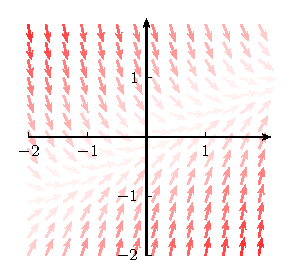
\includegraphics[width=4.6cm]{vecb5}
\hskip1cm\includegraphics[width=4.6cm]{vecb6}
\caption{The vector fields of the equation $y'=x-2y$ with $n_a=\texttt{7pt}$ (the left) and $n_a=\texttt{4pt}$ (the right)}\label{Fig10}
\end{figure}

In Figure \ref{Fig11}, the vector fields of the equations $y'=y-x$ and $y'=x(2-y)$ are respectively drawn by the calling sequences
\begin{verbatim}
\vecfldnew{\nx=-3.00+0.4}{\ny=-3.00+0.4}{15}{15}{0.35}{(\ny)-(\nx)}
{\fy=\ny pt \fx=\nx pt \advance\slope by -\fx \advance\slope by \fy}{5pt}
\end{verbatim}
and
\begin{verbatim}
\vecfldnew{\nx=-3.00+0.4}{\ny=-3.00+0.4}{15}{15}{0.35}{(\nx)*(2-(\ny))}
{\fy=\ny pt \fx=\nx pt \advance\slope by -\decimal\fx\fy
\advance\slope by 2\fx}{6pt}
\end{verbatim}
\begin{figure}[htbp]
\centering\includegraphics[width=6.2cm]{vecb3}
\hskip1cm\includegraphics[width=6.2cm]{vecb4}
\caption{The vector fields of the equation $y'=y-x$ (the left) and $y'=x(2-y)$ (the right).}\label{Fig11}
\end{figure}

Finally, we consider two more examples on vector fields of differential equations $y'=f(x,y)$ containing trigonometric or rational functions on their right side. The calling sequences
\begin{verbatim}
\vecfldnew{\nx=-3.00+0.4}{\ny=-3.00+0.4}{15}{15}{0.35}{sin(\nx)*cos(\ny)}
{\SIN{\nx}{\tmpa}\COS{\ny}{\tmpb}\MULTIPLY{\tmpa}{\tmpb}{\tmpc}
\slope=\tmpc pt}{0.6pt}
\end{verbatim}
and
\begin{verbatim}
\vecfldnew{\nx=-3.00+0.3}{\ny=-3.00+0.3}{20}{20}{0.3}{2*(\nx)*(\ny)/(1+(\ny)^2)}
{\SUMfunction{\ONEfunction}{\SQUAREfunction}{\Fncty}\Fncty{\ny}{\soly}{\Dsoly}
\DIVIDE{\Dsoly}{\soly}{\tempa}\MULTIPLY{\nx}{\tempa}{\tempb}
\slope=\tempb pt}{2.5pt}
\end{verbatim}
respectively result in the vector fields on the left and on the right in Figure \ref{Fig12}.

\begin{figure}[htbp]
\centering\includegraphics[width=6.2cm]{vecb1}
\hskip1cm\includegraphics[width=6.2cm]{vecb2}
\caption{The vector fields of the equation $y'=\sin(x)\cos(y)$ (the left) and $y'=2xy/(1+y^2)$ (the right).}\label{Fig12}
\end{figure}
\section{Drawing partitions of a simply connected plane domain}
\subsection{Description}
B\'{e}zier curves have been used in many different aspects, but mostly in computer graphics to model smooth curves designed by computer
programs. We just recall here the vector function of a B\'{e}zier curve of degree $n$ with $n+1$ control points whose position
vectors are $\mathbf{r}_0$, $\mathbf{r}_1$, \dots, $\mathbf{r}_n$. It is the vector function $\mathbf{r}(t)$ in a real variable $t\in[0,1]$ that
is defined as
\begin{equation}\label{eqn9}
\mathbf{r}(t)=\sum_{i=0}^n\binom{n}{i}t^i(1-t)^{n-i}\mathbf{r}_i.
\end{equation}
Since $\mathbf{r}(0)=\mathbf{r}_0$, $\mathbf{r}(1)=\mathbf{r}_n$ and $\mathbf{r}'(0)=n(\mathbf{r}_1-\mathbf{r}_0)$, $\mathbf{r}'(1)=n(\mathbf{r}_n-\mathbf{r}_{n-1})$,
we can take a curve such that it is closed and tangent to a line $(\Delta)$ at the point whose position vector is $\mathbf{r}_0$, by
letting $\mathbf{r}_n=\mathbf{r}_0$ and the points whose position vectors are $\mathbf{r}_0$, $\mathbf{r}_1$ and $\mathbf{r}_{n-1}$
all be on the line $(\Delta)$.

Taking a closed B\'{e}zier curve to be the boundary of a plane domain has the great advantage. That is because coordinates of points
on the curve are evaluated by polynomials, and the curve has necessary smoothness, beautiful enough for graphic illustrations.
\texttt{PSTricks} has the procedure \verb!\parametricplot! to draw such a curve. But, an important problem here is how to control
the coordinates of its points to construct a procedure for drawing a partition of a simply connected plane domain and coloring
(or marking) its cells having common points with the boundary of the domain. We particularly need such a procedure for illustrations
of essential notions in measure theory or double integral definition. Because of the limitation in accuracy imposed
by the \TeX\ arithmetic, we should mention about $2$-dimension vector functions of a B\'{e}zier curve of small degree (in fact, as small as possible).
According to the above requirements for the closed boundary of a simply connected domain, we will design a family of closed B\'{e}zier curves of
degree $6$, although we may extend their degree to $12$.

From the expression of $\mathbf{r}(t)$ in (\ref{eqn9}), we will construct the following functions and procedures:
\begin{itemize}
\item The factorial function \texttt{FACTORIAL}.
\item The binomial function \texttt{BINOMIAL}.
\item Polynomials $t^m(1-t)^n$.
\item A procedure to compute a sum of $7$ terms: values of $\mathbf{r}(t)$ as linear combinations
of the Bernstein polynomials
$$\binom{6}{k}t^k(1-t)^{6-k},\quad k=0,\ldots,6.$$
\end{itemize}
These functions and procedures are macros given by definitions with or without parameters. In the following subsections we will construct them step by step and
show how to make connections between them.
\subsubsection{Factorial functions and binomial coefficients}
To obtain the factorial function, a procedure for multiplying consecutively an integer $n$ with its diminished values will be constructed. For the declared
integer variables \verb!\Fa! and \verb!\Fct!, the latter will hold values of the function, and the former will hold factors that are multiplied consecutively
and reduced by $1$. Namely, if \verb!\Fa! is $0$ or $1$ then \verb!\Fct! takes $1$; else if $\texttt{\symbol{92}Fa}>1$ then \verb!\Fct! takes
the initial value of \verb!\Fa! to begin a loop: diminishing \verb!\Fa! by $1$ and updating \verb!\Fct! by multiplying its old value with the new value of \verb!\Fa!.
The loop is defined by the control sequence \verb!\Factor! and is ended when \verb!\Fa! is diminished to $1$; then, the factorial function obtains its value from
the one given back after calling \verb!\FACTORIAL! with one parameter.
\begin{verbatim}
\newcount\Fa\newcount\Fct
\newcount\tempA
\def\Factor{\ifnum\Fa=1\relax\else\advance\Fa by -1\multiply\Fct by \Fa\Factor\fi}
\def\FACTORIAL#1{\Fa=#1 \ifnum\Fa=0 \Fct=1\relax\else\Fct=\Fa \Factor\fi%
\global\tempA=\Fct}
\end{verbatim}
Since \TeX\ limits the largest integer number to $2^{30}-1$, we can evaluate only to
$$\textmtt{\symbol{92}FACTORIAL\{$12$\}}=12!=479001600.$$
Besides, the last value of \verb!\Fct!, which is right the one obtained from calling the function, is assigned to a global integer variable \verb!\tempA! for use
in other procedures. Finally, make the calling sequence
$$\textmtt{\symbol{92}FACTORIAL\{k\}\symbol{92}the\symbol{92}Fct}$$
to obtain and show up the value of $k!$. From these values we derive binomial coefficients by the formula
$$\binom{m}{n}=\frac{m!}{n!(m-n)!}.$$
A simple procedure that makes division of $m!$ by $n!$, then of the result by $(m-n)!$ can be performed by the control sequence
\verb!\BINOMIAL! with two parameters as follows
\begin{verbatim}
\newcount\BINOM
\newcount\temp\newcount\tmp
\def\BINOMIAL#1#2{%
\temp=#1\advance\temp by -#2
\FACTORIAL{#1}
\tmp=\tempA
\FACTORIAL{\temp}
\temp=\tempA
\divide\tmp by \temp
\FACTORIAL{#2}
\temp=\tempA
\divide\tmp by \temp\global\BINOM=\tmp}
\end{verbatim}
Again, the last value of \verb!\tmp! is assigned to a global integer variable \verb!\BINOM! for later use. Because the vector function of a B\'{e}zier
curve of degree $6$ is only needed, so are the binomial coefficients \verb!\BINOMIAL{!$6$\verb!}{!$k$\verb!}!, $k=0,1,\ldots,6$.
\subsubsection{Bernstein polynomials}
The construction of Bernstein functions is based on an iterative multiplication of the same value $t$ by a given number $m$ of times,
then the process is repeated with the value $1-t$ by a given number $n$ of times. The last result is multiplied by a variable that holds
the value of $\binom{m+n}{m}$. We will use an integer variable \verb!\kc! to count times of multiplication for the same factor $t$ or $1-t$.
The procedure of iterative multiplication \verb!\xmult! with one parameter $m$ or $n$ is a recursive one that is performed
iteratively until \verb!\kc! reaches the value $m$ or $n$.
\begin{verbatim}
\newdimen\Xa\newdimen\Yb\newcount\kc
\def\xmult#1{\ifnum\kc<#1\advance\kc by 1\Yb=\decimal\Xa\Yb\xmult{#1}
                                                      \else\relax\fi}
\end{verbatim}
Finally, the value of $t^m(1-t)^n$ that is hold by the variable \verb!\Yb! is multiplied by \verb!\BINOM!, the value $\binom{6}{m}$.
Thus, Bernstein polynomials are given by the following macro \verb!\BERNSTEIN! with three parameters that hold values of
$m$, $n$ and $t$, respectively.
\begin{verbatim}
\newdimen\BSTemp
\def\BERNSTEIN#1#2#3{\Xa=#3pt\kc=0\Yb=1pt\xmult{#1}\kc=0\Xa=-\Xa
\advance\Xa by 1pt\xmult{#2}\BINOMIAL{6}{#1}\global\BSTemp=\BINOM\Yb}
\end{verbatim}
Also, values of \verb!\BERNSTEIN! are assigned to a global variable.
\subsubsection{Vector functions of a plane B\'{e}zier curve of degree $6$}
We will construct here the vector function of a plane and closed B\'{e}zier curve with the control points
$M_0(x_0,y_0)$, $M_1(x_1,y_1)$, \dots, $M_6(x_6,y_6)$ that is chosen in such a way that the curve is tangent to
a line $(\Delta)$ at its initial point $M_0$. According to the mentioned properties of a B\'{e}zier curve, the requirements
for the curve are satisfied when $M_6=M_0$ and $M_0$, $M_1$, $M_5$ are all on the line $(\Delta)$.
\begin{figure}[htbp]
\centering\includegraphics[height=4.3cm]{Fig13}
\caption{A B\'{e}zier curve of degree $6$ with the required control points.}\label{Fig13}
\end{figure}
In case $n=6$, from (\ref{eqn9}) we derive the vector function $\mathbf{r}(t)$ with the two components
\begin{equation}\label{eqn10}
X(t)=\sum_{i=0}^6\binom{6}{i}t^i(1-t)^{6-i}x_i,\quad Y(t)=\sum_{i=0}^6\binom{6}{i}t^i(1-t)^{6-i}y_i.
\end{equation}
We first evaluate values of $X(t)$ by the procedures that just have been constructed, with a choice of $x_i$, $i=1,\ldots,6$, from a given $x_0$
and the requirements of the B\'{e}zier curve as in Figure \ref{Fig13}. For example, we may take
$$x_1=x_0-1.5,\quad x_2=x_0+2,\quad x_3=x_0+6,\quad x_4=x_0+5,\quad x_5=x_0+1.5,\quad x_6=x_0.$$
Moreover, we may change the shape of the curve by taking a factor $\alpha$ for $X(t)$. In short, we will make a procedure to evaluate the sum of terms
$\binom{6}{i}t^i(1-t)^{6-i}(\alpha x_i)$, $i=0,1,\ldots,6$. In fact, it is a procedure to add up values into a global variable \verb!\XBST! that is called
by a macro \verb!\XBC! with three declaring parameters for $x_i$, $t$ and $\alpha$. The value of $\alpha$ is used last when being multiplied by a
variable that holds $X(t)$. Such a procedure is suggested to be the following macro
\begin{verbatim}
\newdimen\Xrf\newdimen\Yrf
\newdimen\XBST\newdimen\YBST
\def\XBC#1#2#3{%
\BERNSTEIN{0}{6}{#2}
\Xrf=#1pt
\XBST=\decimal\BSTemp\Xrf
\BERNSTEIN{1}{5}{#2}
\Xrf=#1pt\advance\Xrf by -1.5pt
\advance\XBST by \decimal\BSTemp\Xrf
\BERNSTEIN{2}{4}{#2}
\Xrf=#1pt\advance\Xrf by 2pt
\advance\XBST by \decimal\BSTemp\Xrf
\BERNSTEIN{3}{3}{#2}
\Xrf=#1pt\advance\Xrf by 6pt
\advance\XBST by \decimal\BSTemp\Xrf
\BERNSTEIN{4}{2}{#2}
\Xrf=#1pt\advance\Xrf by 5pt
\advance\XBST by \decimal\BSTemp\Xrf
\BERNSTEIN{5}{1}{#2}
\Xrf=#1pt\advance\Xrf by 1.5pt
\advance\XBST by \decimal\BSTemp\Xrf
\BERNSTEIN{6}{0}{#2}
\Xrf=#1pt
\advance\XBST by \decimal\BSTemp\Xrf
\global\XBST=#3\XBST}
\end{verbatim}
In the macro, a control sequence of the form \verb!\decimal\Xdim! is for obtaining the decimal value of a variable \verb!\Xdim! without units
(\verb!pt!, by default). This can be defined by
\begin{verbatim}
\def\xch{\catcode`\p=12 \catcode`\t=12}\def\ych{\catcode`\p=11 \catcode`\t=11}
\xch \def\dec#1pt{#1}\ych \gdef\decimal#1{\expandafter\dec \the#1}
\end{verbatim}
Besides, the last line in the definition of \verb!\XBC! (\verb!\global\XBST=#3\XBST!) signifies \verb!\XBST! is adjusted for multiplication by
$\alpha$ when holding the current value of the sum $X(t)$. In Table \ref{bc-Table1}, some values
of \verb!\XBC! are compared with those of a simpler procedure in Maple\footnote{\footnotesize Maple
is a computer algebra system. It was first developed in 1980 by the Symbolic Computation Group at the University of
Waterloo in Waterloo, Ontario, Canada. Maple supports numeric and symbolic computations
and can be used as a programming language, which resembles Pascal.}.
\begin{table}[htbp]
\centering\begin{tabular}{|c|c|c|c|c|c|}\hline
&$(-2.4,0.23,1.5)$&$(4.2,0.45,1.1)$&$(-3.4,0.7,1.24)$&$(-0.89,0.4,1.5)$&$(5.21,0.5,2.15)$\\ \hline
\texttt{\symbol{92}XBC}&$\XBC{-2.4}{0.23}{1.5}\decimal\XBST$&$\XBC{4.2}{0.45}{1.1}\decimal\XBST$&$\XBC{-3.4}{0.7}{1.24}\decimal\XBST$&$\XBC{-0.89}{0.4}{1.5}\decimal\XBST$&$\XBC{5.21}{0.5}{2.15}\decimal\XBST$\\ \hline
Maple&$-2.41044$&$8.13235$&$-0.13696$&$2.78628$&$18.76008$\\ \hline
\end{tabular}
\caption{A comparison between some values of \textmtt{\symbol{92}XBC} and those of a procedure in Maple.}\label{bc-Table1}
\end{table}

Likewise, from a given $y_0$, we may have a choice of $y_i$, $i=1,\ldots,6$, as follows
$$y_1=y_0+2,\quad y_2=y_0+5,\quad y_3=y_0+3,\quad y_4=y_0-1,\quad y_5=y_0-2,\quad y_6=y_0.$$
The macro \verb!\YBC! is constructed in a quite analogous way as for \verb!\XBC! to evaluate values of $Y(t)$ in (\ref{eqn10}),
and the value $\beta Y(t)$ ($\beta$ is again an adjustment factor) is hold by a global variable \verb!\YBST!.

\subsubsection{Partition of a simply connected plane domain by a rectangular grid}

We consider here a simply connected plane domain $D$ surrounded by a B\'{e}zier curve of degree $6$ that will be depicted by
the procedure \verb!\NetDraw!. This is called together with its five parameters whose values are assigned to the five local variables
with their following meaning:
\begin{align*}
\texttt{\symbol{92}CellNum:}&\text{ The number of horizontal and vertical cells of the grid.}\\
\texttt{\symbol{92}Xref:}&\text{ The value of $x_0$.}\\
\texttt{\symbol{92}Yref:}&\text{ The value of $y_0$.}\\
\texttt{\symbol{92}Xfact:}&\text{ The value of $\alpha$.}\\
\texttt{\symbol{92}Yfact:}&\text{ The value of $\beta$.}
\end{align*}
We denote by $R$ a rectangular domain containing $D$ and having edges parallel to the coordinate axes.
A grid of rectangular cells will be depicted on $R$. According to the given values of $x_0$, $y_0$, $\alpha$ and $\beta$, the vertices of $R$
can be chosen as the points  $(\verb!\XMin!,\verb!\YMax!)$, $(\verb!\XMax!,\verb!\YMax!)$, $(\verb!\XMax!,\verb!\YMin!)$, $(\verb!\XMin!,\verb!\YMin!)$, where
\begin{align*}
\textmtt{\symbol{92}XMin}&=\alpha(\textmtt{\symbol{92}Xref}-1.5),&&\textmtt{\symbol{92}XMax}=\alpha(\textmtt{\symbol{92}Xref}+6),\\
\textmtt{\symbol{92}YMin}&=\beta(\textmtt{\symbol{92}Yref}-2),&&\textmtt{\symbol{92}YMax}=\beta(\texttt{\symbol{92}Yref}+5).
\end{align*}
Then, the horizontal step size \verb!\Xsize! and the vertical step
size \verb!\Ysize! may be taken as
$$\mtt\\\texttt{Xsize}=\frac{\mtt\\\texttt{XMax}-\mtt\\\texttt{XMin}}{\mtt\\\texttt{CellNum}},\quad
\mtt\\\texttt{Ysize}=\frac{\mtt\\\texttt{YMax}-\mtt\\\texttt{YMin}}{\mtt\\\texttt{CellNum}}.$$

At first, the grid is made by using the structure \verb!\multido! to draw vertical and horizontal lines whose equations are
$$x=\texttt{\symbol{92}XMin}+i\texttt{\symbol{92}Xsize},\quad
y=\texttt{\symbol{92}YMin}+i\texttt{\symbol{92}Ysize},\quad i=0,\ldots,\texttt{\symbol{92}CellNum}.$$
Next, the B\'{e}zier curve is depicted by the command
$$\textmtt{\symbol{92}parametricplot[algebraic,fillstyle=solid]\{$0$\}\{$1$\}\{$\alpha X(t)$|$\beta Y(t)$\}}$$
and it is approximated by the sequence of points $(X_i,Y_i)$, $i=1,\ldots,N$, where $X_i$ and $Y_i$ are given from
the calling sequences
$$\textmtt{\symbol{92}XBC\{\symbol{92}XRef\}\{$t_i$\}\{\symbol{92}Xfact\}},\quad
\textmtt{\symbol{92}YBC\{\symbol{92}YRef\}\{$t_i$\}\{\symbol{92}Yfact\}}.$$

Finally, the most important algorithm is to determine cells that have points in common with the B\'{e}zier curve,
and to color them. The chosen ``filter'' method here can be described as follows: for each point $(X_i,Y_i)$ of the approximate sequence,
$i=1,\ldots, N$, we examine cells from left to right in horizontal direction, and from below to above in vertical direction. As soon as
being found, the cell containing $(X_i,Y_i)$ is specifically colored by the command \textmtt{\mtt\\pspolygon[fillstyle=solid,$\ldots$]} passing its four
vertices; then, we examine the next point $(X_{i+1},Y_{i+1})$, and so on. Actually, a structure of three nested \verb!\multido! loops
is used to perform this filter method, and the loop for counting points $(X_i,Y_i)$ is the most outer one. The algorithm to examine if
a cell contains $(X_i,Y_i)$ may have the form of
\begin{verbatim}
     \ifdim\YBST<y\relax\else\advance y by \Ysize
      \ifdim\YBST>y\relax\else
       \ifdim\XBST<x\relax\else\advance x by \Xsize
        \ifdim\XBST>x\relax\else
         \pspolygon[fillstyle=solid,fillcolor=red]
           (x,y)(x+\Xsize,y)(x+\Xsize,y+\Ysize)(x,y+\Ysize)(x,y)\relax
            \fi\fi\fi\fi
\end{verbatim}
The single characters ``\verb!x!'', ``\verb!y!'' and the opertation ``\verb!+!'' will be replaced appropriately in the procedure \verb!\NetDraw! below.
For increasingly chosen values of $N$, we may know if the set of cells having points in common with the curve can cover the curve itself?
On the other hand, to increase the number of approximate points is corresponding to reduce the increment in the most outer loop \verb!\multido!.
For instance, if we take $N=100$, then the variable \verb!\nz! in the loop should be declared as $\texttt{\mtt\\nz}=0.00+0.01$ because
$t_i\in[0,1]$.

In summary, to illustrate a partition of a simply connected plane domain, we can apply the following procedure \verb!\NetDraw!. As mentioned above,
step by step, \verb!\NetDraw! can: draw the boundary of a plane domain $D$ by a B\'{e}zier curve of degree $6$, draw a partition of a rectangle $R$ containing $D$
by a grid of rectangular cells, and color cells having points in common with the boundary of $D$.
\bigskip
%\vskip2ex
\hrule
\begin{verbatim}
\def\NetDraw#1#2#3#4#5{%
\newcount\CellNum
\newdimen\XRef
\newdimen\YRef
\newdimen\Xfact
\newdimen\Yfact
\newdimen\XMin
\newdimen\XMax
\newdimen\YMin
\newdimen\YMax
\newdimen\Xsize
\newdimen\Ysize
\newdimen\tempx
\newdimen\tempy
\CellNum=#1
\XRef=#2pt
\YRef=#3pt
\Xfact=#4pt
\Yfact=#5pt
\XMin=\decimal\Xfact\XRef \advance\XMin by -1.50\Xfact
\XMax=\decimal\Xfact\XRef \advance\XMax by 6.00\Xfact
\YMin=\decimal\Yfact\YRef \advance\YMin by -2.00\Yfact
\YMax=\decimal\Yfact\YRef \advance\YMax by 5.00\Yfact
\Xsize=\XMax \advance\Xsize by -\XMin \divide\Xsize by \CellNum
\Ysize=\YMax \advance\Ysize by -\YMin \divide\Ysize by \CellNum
\parametricplot[algebraic,fillstyle=solid,fillcolor=yellow!80,plotpoints=200,
linewidth=0.5pt]{0}{1}{\XBsix{\decimal\XRef}{\decimal\Xfact}|
\YBsix{\decimal\YRef}{\decimal\Yfact}}
\multido{\nz=0.00+0.005}{200}{\XBC{\decimal\XRef}{\nz}{\decimal\Xfact}
\YBC{\decimal\YRef}{\nz}{\decimal\Yfact}
\multido{\nx=\decimal\XMin+\decimal\Xsize}{\the\CellNum}
{\tempx=\nx pt\multido{\ny=\decimal\YMin+\decimal\Ysize}{\the\CellNum}
{\tempy=\ny pt\ifdim\YBST<\tempy\relax\else\advance\tempy by \Ysize%
              \ifdim\YBST>\tempy\relax\else
              \ifdim\XBST<\tempx\relax\else\advance\tempx by \Xsize
              \ifdim\XBST>\tempx\relax\else
              \pspolygon[fillstyle=solid,fillcolor=blue!90,linecolor=black,
              linewidth=0.2pt]
              (\nx,\ny)(\decimal\tempx,\ny)(\decimal\tempx,\decimal\tempy)
              (\nx,\decimal\tempy)(\nx,\ny)\relax\fi\fi\fi\fi}
}}
\advance\CellNum by 1
\multido{\nx=\decimal\XMin+\decimal\Xsize}{\the\CellNum}
{\psline[linewidth=0.2pt](\nx,\decimal\YMax)(\nx,\decimal\YMin)}
\multido{\ny=\decimal\YMin+\decimal\Ysize}{\the\CellNum}
{\psline[linewidth=0.2pt](\decimal\XMin,\ny)(\decimal\XMax,\ny)}
\parametricplot[algebraic,linecolor=white,plotpoints=200,linewidth=0.5pt]{0}{1}
{\XBsix{\decimal\XRef}{\decimal\Xfact}|\YBsix{\decimal\YRef}{\decimal\Yfact}}}
\end{verbatim}\hrule\bigskip

In the definition of \verb!\NetDraw!, the expressions $\alpha X(t)$, $\beta Y(t)$ are declared in the \verb!algebraic! form by the macros \verb!\XBsix!,
\verb!\YBsix! with two parameters that hold values of $x_0,\alpha$ and $y_0,\beta$, respectively. These macros are given by
the following definitions:
\begin{verbatim}
\def\XBsix#1#2{%
(1-t)^6*(#1)*(#2)+6*t*(1-t)^5*(#1-1.5)*(#2)+15*t^2*(1-t)^4*(#1+2)*(#2)+
20*t^3*(1-t)^3*(#1+6)*(#2)+15*t^4*(1-t)^2*(#1+5)*(#2)+
6*t^5*(1-t)*(#1+1.5)*(#2)+t^6*(#1)*(#2)}
\def\YBsix#1#2{%
(1-t)^6*(#1)*(#2)+6*t*(1-t)^5*(#1+2)*(#2)+15*t^2*(1-t)^4*(#1+5)*(#2)+
20*t^3*(1-t)^3*(#1+3)*(#2)+15*t^4*(1-t)^2*(#1-1)*(#2)+
6*t^5*(1-t)*(#1-2)*(#2)+t^6*(#1)*(#2)}
\end{verbatim}
\subsection{Examples}
Firstly, let us see the effect of change for the shape of a domain when adjusting its boundary by taking different values of $\alpha$ and $\beta$. The
calling sequence for this purpose may have the form of
\begin{align*}
&\textmtt{\mtt\\parametricplot[algebraic,plotpoints=200,linewidth=0.5pt]\{$0$\}\{$1$\}}\\
&\textmtt{\mtt\{XBsix\{$x_0$\}\{$\alpha$\}|\mtt\\YBsix\{$y_0$\}\{$\beta$\}\mtt\}}
\end{align*}
and its result is given in Figure \ref{Fig14}.
\begin{figure}[htbp]
\centering\includegraphics[height=3cm]{Fig14}
\caption{From left to right, corresponding to the couple of values:
$\alpha=2,\,\beta=2$; $\alpha=2.5,\,\beta=2$; $\alpha=2,\,\beta=2.5$.}\label{Fig14}
\end{figure}

The Table \ref{bc-table2} below provides three partitions of a domain $D$ with cells that decrease in size. In each case, \verb!\NetDraw! can
determine the cells that have points in common with the boundary curve and color them. The calling sequence here
takes a simple form
$$\textmtt{\mtt\\NetDraw\{$c$\}\{$x_0$\}\{$y_0$\}\{$\alpha$\}\{$\beta$\}}$$
The numerical argument $c$ is assigned to the local variable \verb!\CellNum!. The number of approximate points $(X_i,Y_i)$ for the boundary curve
is chosen to be $200$, by default, corresponding to the increment $\Delta\mtt{z}=0.005$. The number $N$ can be made larger and the filter procedure
for determining required cells may be more exact. In Table \ref{bc-table2}, the B\'{e}zier curves are depicted with the choice
$x_0=y_0=\alpha=\beta=2$.
\begin{table}[htbp]
\centering\begin{tabular}{cc}
\includegraphics[width=6cm]{b6of1}&\includegraphics[width=6cm]{b6of2}\\
\includegraphics[width=6cm]{b6of3}&\includegraphics[width=6cm]{b6of4}
\end{tabular}
\caption{The partitions of $D$ with $c=18$, $c=36$ and $c=63$.}\label{bc-table2}
\end{table}

\acknw
I am very grateful to
\begin{itemize}
\item Timothy Van Zandt, Herbert Vo\ss, Dominique Rodriguez and Michael Sharpe for helping me with
their great works on \texttt{PSTricks}.
\item H\`an Th\hantt\rlap\accentcircflx\ Th\`anh for helping me with his pdf\hskip.03em\LaTeX\ program.
\item Robert Fuster for his very useful package \texttt{calculator}.
\end{itemize}
\begin{thebibliography}{10}
\bibitem{one} Dominique Rodriguez, Michael Sharpe \&\ Herbert Vo\ss. \textsl{\texttt{pstricks-add}: Additional Macros for PSTricks\/}.
Version 3.60,
\url{http://ctan.org/tex-archive/graphics/pstricks/contrib}, 2013
\bibitem{two} Timothy Van Zandt, Michael Sharpe \&\ Herbert Vo\ss. \textsl{\texttt{pst-node}: Nodes and node connections}.
Version 1.29,
\url{http://ctan.org/tex-archive/graphics/pstricks/contrib}, 2013
\bibitem{three} Helmut Kopka \&\ Patrick W. Daly. \textsl{Guide to \LaTeX \/}.
Addison-Wesley, Fourth Edition, 2004, ISBN 0321173856
\bibitem{four} Timothy Van Zandt. \textsl{User's Guide\/}. Version 1.5,\\
\url{http://ctan.org/tex-archive/graphics/pstricks/base}, 2007
\bibitem{five}Eitan M. Gurari. \textsl{Writing With \TeX \/}, McGraw-Hill, Inc., 1994, ISBN 0-07-025207-6
\bibitem{six} Robert Fuster. \textsl{\texttt{calculator-calculus}: Scientific Calculations With \LaTeX \/}. Version 1.0a,
\url{http://ctan.org/tex-archive/macros/latex/contrib/calculator}, 2012
\end{thebibliography}

\end{document}
\begin{thebibliography}{10}
\bibitem{one} Dominique Rodriguez, Michael Sharpe \&\ Herbert Vo\ss. \textsl{\texttt{pstricks-add}: Additional Macros for PSTricks\/}.
Version 3.60,
\url{http://ctan.org/tex-archive/graphics/pstricks/contrib}, 2013
\bibitem{two} Timothy Van Zandt, Michael Sharpe \&\ Herbert Vo\ss. \textsl{\texttt{pst-node}: Nodes and node connections}.
Version 1.29,
\url{http://ctan.org/tex-archive/graphics/pstricks/contrib}, 2013
\bibitem{three} Helmut Kopka \&\ Patrick W. Daly. \textsl{Guide to \LaTeX \/}.
Addison-Wesley, Fourth Edition, 2004, ISBN 0321173856
\bibitem{four} Timothy Van Zandt. \textsl{User's Guide\/}. Version 1.5,\\
\url{http://ctan.org/tex-archive/graphics/pstricks/base}, 2007
\bibitem{five}Eitan M. Gurari. \textsl{Writing With \TeX \/}, McGraw-Hill, Inc., 1994, ISBN 0-07-025207-6
\bibitem{six} Robert Fuster. \textsl{\texttt{calculator-calculus}: Scientific Calculations With \LaTeX \/}. Version 1.0a,
\url{http://ctan.org/tex-archive/macros/latex/contrib/calculator}, 2012
\end{thebibliography}
